\documentclass[a4paper,11pt,reqno]{amsart}

% --------------------------------------------------------
% Packages
% --------------------------------------------------------
\usepackage[utf8]{inputenc}
\usepackage[foot]{amsaddr}
\usepackage{amsmath,amsfonts,amssymb,amsthm,mathrsfs,bm}
\usepackage[margin=0.95in]{geometry}
\usepackage{color}
\usepackage[dvipsnames]{xcolor}
\usepackage{mathtools,graphicx}
\usepackage{tcolorbox}
\usepackage{listings}
\usepackage{textcomp}
\usepackage{units}
\usepackage{cite}
\usepackage{hyperref}
\usepackage{subfigure} % 支持多图
\usepackage{float}
\usepackage{overpic}

% --------------------------------------------------------
% Custom Colours
% --------------------------------------------------------
\definecolor{CommentGreen}{rgb}{0.0,0.4,0.0}
\definecolor{Background}{rgb}{0.9,1.0,0.85}
\definecolor{lrow}{rgb}{0.914,0.918,0.922}
\definecolor{drow}{rgb}{0.725,0.745,0.769}


% --------------------------------------------------------
% Typesetting Python code
% --------------------------------------------------------
\lstloadlanguages{Python}%
\lstset{
    language=Python, upquote=true, frame=single,
    basicstyle=\small\ttfamily,
    backgroundcolor=\color{yellow!30},
    keywordstyle=[1]\color{NavyBlue}\bfseries,
    keywordstyle=[2]\color{RubineRed},
    keywordstyle=[3]\color{orange!90}\bfseries,
    keywordstyle=[4]\color{Green!90}\bfseries,
    identifierstyle=,
    commentstyle=\usefont{T1}{pcr}{m}{sl}\color{MidnightBlue}\small,
    stringstyle=\color{purple},
    showstringspaces=false, tabsize=4, morekeywords={import,as},
    morekeywords=[2]{args,__init__},
    morekeywords=[3]{@property},
    morekeywords=[4]{self},
    morecomment=[l][\color{blue}]{...},
    numbers=none, firstnumber=1,
    numberstyle=\tiny\color{blue},
    stepnumber=1, xleftmargin=10pt, xrightmargin=10pt
}

\synctex=1

\hypersetup{
    unicode=false, pdftoolbar=true, 
    pdfmenubar=true, pdffitwindow=false, pdfstartview={FitH}, 
    pdftitle={ELE8088 Coursework}, pdfauthor={A. Author},
    pdfsubject={ELE8088 coursework}, pdfcreator={A. Author},
    pdfproducer={ELE8088}, pdfnewwindow=true,
    colorlinks=true, linkcolor=red,
    citecolor=blue, filecolor=magenta, urlcolor=cyan
}

% --------------------------------------------------------
% CUSTOM COMMANDS
% --------------------------------------------------------
\newcommand{\iu}{{\mathrm{i}\mkern1mu}}
\newcommand{\R}{{\rm I\!R}}
\newcommand{\N}{{\rm I\!N}}
\newcommand{\E}{{\rm I\!E}}
\newcommand{\C}{\mathbb{C}}
\newcommand{\dd}{\mathrm{d}}
\newcommand{\tran}{\intercal}
\DeclareMathOperator{\Var}{Var}
\DeclareMathOperator*{\argmin}{arg\,min}
\DeclareMathOperator*{\argmax}{arg\,max}
\DeclareMathOperator*{\minimise}{minimise}
\newcommand{\smallmat}[1]{\left[ \begin{smallmatrix}#1 \end{smallmatrix} \right]}
\newcommand{\smallplus}{{\scriptscriptstyle +}}
\newcommand{\Spp}{\mathbb{S}_{\smallplus\smallplus}}
\newcommand{\Sp}{\mathbb{S}_{\smallplus}}
\newcommand{\prob}{\mathrm{P}}
\renewcommand{\thefootnote}{\fnsymbol{footnote}}

% --------------------------------------------------------
% Opening: Title and Author Names
%          Modify this section
% --------------------------------------------------------
\title[ELE8088 Coursework]{Control \& Estimation Theory}

\author[Z. Zhang]{Zichi Zhang}
\author[S. Chen]{Shihao Chen}
\address[Zichi Zhang and Shihao Chen]{Email addresses: \href{mailto:zzhang54@qub.ac.uk}%
{zzhang54@qub.ac.uk} and 
\href{mailto:schen45.ac.uk}{schen45@qub.ac.uk}.}
\thanks{Thanks Dr. Pantelis Sopasakis. Version 1.0.1. Last updated:~\today.}



% --------------------------------------------------------
% Beginning of your document
% --------------------------------------------------------
\begin{document}

\maketitle



% --------------------------------------------------------
% Section 1: Control
% --------------------------------------------------------
\section{Part I: Control}


% Subsection: Optimal Control
% ^^^^^^^^^^^^^^^^^^^^^^^^^^^
\subsection*{1.1 Optimal Control}\label{sec:q1}
\
\\ \\
(i) Prove that the function $g:\R^n\to \R$ given by $g(x) = \frac{1}{2}x^{\tran}Qx+q^{\tran}x+c$ with $Q\in \mathbb{S}^n_+$ is level-bounded
if and only if $Q\in \mathbb{S}^n_{++}$.
\\ \\
\textbf{Proof:}
\begin{align}
    \mathrm{lev}_{\leq \alpha}f&=\{x\in\R^n:f(x)\leq\alpha\}\notag\\
    &=\{x\in\R^n:x^{\tran}Qx\leq\alpha\}
\end{align}
We are trying to prove that $\mathrm{lev}_{\leq \alpha}f$ are bounded, i.e., there is an $M\geq 0$ such that
\begin{equation}
    \{x\in\R^n:x^{\tran}Qx\leq\alpha\}\subseteq \mathcal{B}_M
\end{equation}
\begin{equation}
    \lambda_{\mathrm{min}}(Q)\left\lVert x\right\rVert ^2\leq x^{\tran}Qx\leq \lambda_{\mathrm{max}}(Q)\left\lVert x\right\rVert ^2
\end{equation}
\begin{align}
    \Longrightarrow &\lambda_{\mathrm{min}}(Q)\left\lVert x\right\rVert ^2\leq \alpha\\
    \Longrightarrow &\left\lVert x\right\rVert \leq \sqrt{\frac{\alpha}{\lambda_{\mathrm{min}}(Q)}}:=M
\end{align}
Thus, if $M\geq 0$ exists, then
\begin{align}
    &\lambda_{\mathrm{min}}(Q)\geq 0\\
    \Longrightarrow&\lambda(Q)\geq 0\\
    \Longrightarrow &Q\in \mathbb{S}^n_{++}
\end{align}
Conclusion: the function $g:\R^n\to \R$ given by $g(x) = \frac{1}{2}x^{\tran}Qx+q^{\tran}x+c$ with $Q\in \mathbb{S}^n_+$ is level-bounded
if and only if $Q\in \mathbb{S}^n_{++}$.
\\ \\
Next, consider the finite-horizon linear-quadratic optimal control problem
\begin{subequations}
    \begin{align}
        \mathbb{P}_N(x): \minimise_{\substack{u_0,u_1,\ldots,u_{N-1}\\ x_0,x_1,\ldots,x_N}} \,
         & \sum_{t=0}^{N-1}\textstyle\frac{1}{2}
         \begin{bmatrix}
             x_t\\
             u_t
         \end{bmatrix}^{\tran}
         \begin{bmatrix}
             Q&S\\
             S^{\tran}&R
         \end{bmatrix}
         \begin{bmatrix}
             x_t\\
             u_t
         \end{bmatrix}
         +\frac{1}{2}x_N^{\tran}P_fx_N,
        \\
        \text{subject to: }\,
         & x_{t+1} = A x_t + B u_t, \forall t\in\N_{[0, N-1]},
        \\
         & x_{0} = x,
    \end{align}
\end{subequations}
where $\begin{bsmallmatrix}Q&S\\S^{\tran}&R\end{bsmallmatrix}\succcurlyeq 0, Q\in \mathbb{S}^n_+, R\in \mathbb{S}^m_{++}, P_f\in \mathbb{S}^n_{+}$, and $x$ is a given initial state.
\\ \\
(ii) Is Problem $\mathbb{P}_N$ convex? Does $\mathbb{P}_N$ have a minimiser?
\\ \\
\textbf{Answer:} Problem $\mathbb{P}_N$ is convex. Problem $\mathbb{P}_N$ has a minimiser.
\\ \\
(iii) Solve Problem $\mathbb{P}_N$ by eliminating the state sequence: determine the optimal sequence of control actions, the optimal sequence(s) of states and the optimal cost.
\\ \\
\textbf{Solusion:}
\\ \\
(iv) Solve Problem $\mathbb{P}_N$ by using the dynamic programming method.
\\ \\
\textbf{Solusion:}
\begin{align}
    &
    \begin{bmatrix}
        x_t\\
        u_t
    \end{bmatrix}^{\tran}
    \begin{bmatrix}
        Q&S\\
        S^{\tran}&R
    \end{bmatrix}
    \begin{bmatrix}
        x_t\\
        u_t
    \end{bmatrix}\notag\\
    &=x_t^{\tran}Qx_t+u_tRu_t+x_t^{\tran}Su_t+u_t^{\tran}S^{\tran}x_t\notag\\
    &=x_t^{\tran}Qx_t+u_tRu_t+x_t^{\tran}Su_t+u_t^{\tran}S^{\tran}x_t+x_t^{\tran}SR^{-1}S^{\tran}x_t-x_t^{\tran}SR^{-1}S^{\tran}x_t\notag\\
    &=x_t^{\tran}(Q-SR^{-1}S^{\tran})x_t+(u_t+R^{-1}S^{\tran}x_t)^{\tran}R(u_t+R^{-1}S^{\tran}x_t)
    \label{eq:P_N_matrix_rewrite}
\end{align}
Let
\begin{equation}
    \begin{cases}
        \tilde{Q}=Q-SR^{-1}S^{\tran}\\
        \tilde{u}_t=u_t+R^{-1}S^{\tran}x_t
    \end{cases}
    \label{eq:tilde_Q_u}
\end{equation}
\begin{align}
    x_{t+1}&=Ax+B(\tilde{u}_t-R^{-1}S^{\tran}x_t)\notag\\
    &=(A-BR^{-1}S^{\tran})x_t+B\tilde{u}_t, \forall t\in\N_{[0, N-1]}
    \label{eq:tilde_x}
\end{align}
Let
\begin{equation}
    \tilde{A}=A-BR^{-1}S^{\tran}
    \label{eq:tilde_A}
\end{equation}
The problem changes to 
\begin{subequations}
    \begin{align}
        \mathbb{P}_N(x): \minimise_{\substack{u_0,u_1,\ldots,u_{N-1}\\ x_0,x_1,\ldots,x_N}} \,
         & \sum_{t=0}^{N-1}\left(\textstyle\frac{1}{2}
         x_t^{\tran}\tilde{Q}x_t+\tilde{u}_t^{\tran}R\tilde{u}_t\right) 
         +\frac{1}{2}x_N^{\tran}P_fx_N,
        \\
        \text{subject to: }\,
         & x_{t+1} = \tilde{A}x_t+B\tilde{u}_t, \forall t\in\N_{[0, N-1]},
        \\
         & x_{0} = x,
    \end{align}
\end{subequations}
where $Q\in \mathbb{S}^n_+, R\in \mathbb{S}^m_{++}, P_f\in \mathbb{S}^n_{+}, \tilde{Q}=Q-SR^{-1}S^{\tran}, \tilde{u}_t=u_t+R^{-1}S^{\tran}x_t, \tilde{A}=A-BR^{-1}S^{\tran}$, and $x$ is a given initial state.
\\ \\
We identify the terminal cost, the stage cost, and the system dynamics. We have
\begin{align}
    V_f(x)&=\textstyle\frac{1}{2}x^{\tran}P_fx,\\
    \ell(x,\tilde{u})&=\textstyle\frac{1}{2}x^{\tran}\tilde{Q}x+\tilde{u}^{\tran}R\tilde{u},\\
    f(x,\tilde{u})&=\tilde{A}x+B\tilde{u}.
\end{align}
We define $V_{0}^{\star}(x)=V_f(x)$, i.e.,
\begin{equation}
    V_{0}^{\star}(x)=\textstyle\frac{1}{2}x^{\tran}P_fx.
\end{equation}
Then, we know that $V_{t+1}^{\star}(x)=(\mathbb{T}V_t^{\star})(x)$. We assume that
\begin{equation}
    V_t^{\star}(x)=\textstyle\frac{1}{2}x^{\tran}P_tx.
\end{equation}
We have
\begin{align} 
    V_t^{\star}(x)&=(\mathbb{T}V_t^{\star})(x)=\min_{\tilde{u}}\left\{\ell(x,\tilde{u})+V_t^{\star}(f(x,\tilde{u}))\right\} \notag\\
    &=\min_{\tilde{u}}\left\{\textstyle\frac{1}{2}x^{\tran}\tilde{Q}x+\tilde{u}^{\tran}R\tilde{u}+\frac{1}{2}(\tilde{A}x+B\tilde{u})^{\tran}P_t(\tilde{A}x+B\tilde{u})\right\}.
\end{align}
After some algebraic manipulations
\begin{equation}
    V_{t+1}^{\star}(x)=\textstyle\frac{1}{2}x^{\tran}(\tilde{Q}+\tilde{A}^{\tran}P_t\tilde{A})x+\min_{\tilde{u}}\left\{\textstyle\frac{1}{2}\tilde{u}^{\tran}(R+B^{\tran}P_tB)\tilde{u}+(B^{\tran}P_t\tilde{A}x)^{\tran}\tilde{u}\right\}.
    \label{eq:V_t+1(x)}
\end{equation}
The minimiser is...
\begin{equation}
    \kappa_{t+1}^{\star}(x)=-(R+B^{\tran}P_tB)^{-1}B^{\tran}P_tAx.
\end{equation}
It is convenient to write $\kappa^{\star}_{t+1}$ as an affine function, i.e., $\kappa_{t+1}^{\star}(x)=K_{t+1}x$, where $K_{t+1}$ is given by
\begin{equation}
    K_{t+1}=-(R+B^{\tran}P_tB)^{-1}B^{\tran}P_tA.
\end{equation}
We can then substitute $\tilde{u}=\kappa_{t+1}^{\star}$ in Equation \eqref{eq:V_t+1(x)}:
\begin{align}
    V_{t+1}^{\star}(x)&=\textstyle\frac{1}{2}x^{\tran}(\tilde{Q}+\tilde{A}^{\tran}P_t\tilde{A})x+\min_{\tilde{u}}\left\{\textstyle\frac{1}{2}\tilde{u}^{\tran}(R+B^{\tran}P_tB)\tilde{u}+(B^{\tran}P_t\tilde{A}x)^{\tran}\tilde{u}\right\}\notag\\
    &=\textstyle\frac{1}{2}x^{\tran}(\tilde{Q}+\tilde{A}^{\tran}P_t\tilde{A})x+\frac{1}{2}(K_{t+1}x)^{\tran}(R+B^{\tran}P_tB)(K_{t+1}x)+(B^{\tran}P_t\tilde{A}x)^{\tran}(K_{t+1}x).
\end{align}
and we can rearrange the terms to write $V_{t+1}^{\star}$ in the form $V_{t+1}^{\star}(x)=\textstyle\frac{1}{2}x^{\tran}P_{t+1}x$.\\
We find that
\begin{equation}
    P_{t+1}=\tilde{Q}+\tilde{A}^{\tran}P_t\tilde{A}+K_{t+1}^{\tran}(R_t+B^{\tran}P_tB)K_{t+1}+2\tilde{A}^{\tran}P_t^{\tran}BK_{t+1}.
\end{equation}
We have that
\begin{equation}
    V_{N}^{\star}(x)=\textstyle\frac{1}{2}x^{\tran}P_Nx.
\end{equation}
We have
\begin{align}
    x_0^{\star}=&x,\notag\\
    \tilde{u}_0^{\star}=&\kappa_N^{\star}(x_0^{\star})=K_Nx_0^{\star},\notag\\
    x_1^{\star}=&\tilde{A}x_0^{\star}+B\tilde{u}_0^{\star},\notag\\
    \tilde{u}_1^{\star}=&\kappa_{N-1}^{\star}(x_1^{\star})=K_{N-1}x_1^{\star},\notag\\
    x_2^{\star}=&\tilde{A}x_1^{\star}+B\tilde{u}_1^{\star},\notag\\
    &\vdots \notag\\
    \tilde{u}_{N-1}^{\star}=&\kappa_1^{\star}(x_{N-1}^{\star})=K_1x_{N-1}^{\star},\notag\\
    x_N^{\star}=&\tilde{A}x_{N-1}^{\star}+B\tilde{u}_{N-1}^{\star}.\notag
\end{align}
\
\\
Next, consider the following infinite-horizon optimal control problem
\begin{subequations}
    \begin{align}
        \mathbb{P}_{\infty}(x): \minimise_{(u_t)_{t\in \N},(x_t)_{t\in \N}} \,
        & \sum_{t=0}^{\infty}\textstyle\frac{1}{2}
        \begin{bmatrix}
            x_t\\
            u_t
        \end{bmatrix}^{\tran}
        \begin{bmatrix}
            Q&S\\
            S^{\tran}&R
        \end{bmatrix}
        \begin{bmatrix}
            x_t\\
            u_t
        \end{bmatrix},
        \\
        \text{subject to: }\,
        & x_{t+1} = A x_t + B u_t, t\in\N,
        \\
        & x_{0} = x,
    \end{align}
\end{subequations}
where $\begin{bsmallmatrix}Q&S\\S^{\tran}&R\end{bsmallmatrix}\succcurlyeq 0, Q\in \mathbb{S}^n_+, R\in \mathbb{S}^m_{++}$.
\\ \\
(v) Under what conditions do the dynamic programming iterates, $V^{\star}_t$, converge? Justify your answer.
\\ \\
\textbf{Anwser:} In order for the dynamic programming iterates, $V^{\star}_t$, converge, it is necessary that there is a sequence of inputs $(u_t)_{t\in \N}$, such that the corresponding states, $(x_t)_{t\in \N}$, are such that the cost function is finite
\begin{equation}
    \sum_{t=0}^{\infty}\textstyle\frac{1}{2}
        \begin{bmatrix}
            x_t\\
            u_t
        \end{bmatrix}^{\tran}
        \begin{bmatrix}
            Q&S\\
            S^{\tran}&R
        \end{bmatrix}
        \begin{bmatrix}
            x_t\\
            u_t
        \end{bmatrix}
    <\infty
\end{equation}
We denote the value function of $\mathbb{P}_{\infty}(x)$ by $V_{\infty}^{\star}(x)$, that is
\begin{equation}
    V_{\infty}^{\star}(x)=\inf_{(u_t)_{t\in \N},(x_t)_{t\in \N}}
    \left\{
    \sum_{t=0}^{\infty}\tfrac{1}{2}
        \begin{bmatrix}
            x_t\\
            u_t
        \end{bmatrix}^{\tran}
        \begin{bmatrix}
            Q&S\\
            S^{\tran}&R
        \end{bmatrix}
        \begin{bmatrix}
            x_t\\
            u_t
        \end{bmatrix}
        \left\lvert
            x_{t+1}=Ax_t+Bu_t,\forall t\in\N,\atop
            x_0=x
        \right. 
    \right\} 
\end{equation}
The value function $V^{\star}_{\infty}$, if it exists, must satisfy $V^{\star}_{\infty}=\mathbb{T}V^{\star}_{\infty}$, which can be equivalently written as
\begin{equation}
    V_{\infty}^{\star}(x)=\min_u
    \left\{
    \sum_{t=0}^{\infty}\tfrac{1}{2}
        \begin{bmatrix}
            x_t\\
            u_t
        \end{bmatrix}^{\tran}
        \begin{bmatrix}
            Q&S\\
            S^{\tran}&R
        \end{bmatrix}
        \begin{bmatrix}
            x_t\\
            u_t
        \end{bmatrix}
        +V_{\infty}^{\star}(x)(Ax+Bu)
    \right\} 
\end{equation}
By Equations \eqref{eq:P_N_matrix_rewrite}, \eqref{eq:tilde_Q_u}, \eqref{eq:tilde_x} and \eqref{eq:tilde_A}, the problem changes to 
\begin{subequations}
    \begin{align}
        \mathbb{P}_{\infty}(x): \minimise_{(u_t)_{t\in \N},(x_t)_{t\in \N}} \,
         & \sum_{t=0}^{\infty}\left(\textstyle\frac{1}{2}
         x_t^{\tran}\tilde{Q}x_t+\tilde{u}_t^{\tran}R\tilde{u}_t\right),
        \\
        \text{subject to: }\,
         & x_{t+1} = \tilde{A}x_t+B\tilde{u}_t, t\in\N,
        \\
         & x_{0} = x,
    \end{align}
\end{subequations}
where $Q\in \mathbb{S}^n_+, R\in \mathbb{S}^m_{++}, \tilde{Q}=Q-SR^{-1}S^{\tran}, \tilde{u}_t=u_t+R^{-1}S^{\tran}x_t, \tilde{A}=A-BR^{-1}S^{\tran}$.
\\ \\
We have known a matrix $P$ satisfying
\begin{equation}
    P=Q+A^{\tran}(P-PB(R+B^{\tran}PB)^{-1}B^{\tran}P)A,
    \tag{DARE}
    \label{eq:DARE}
\end{equation}
which is known a \emph{discrete algebraic Riccati equation} \eqref{eq:DARE}, and
\begin{equation}
    V^{\star}_{\infty}=\tfrac{1}{2}x^{\tran}Px.
\end{equation}
In $\mathbb{P}_{\infty}(x)$, we have
\begin{equation}
    P=\tilde{Q}+\tilde{A}^{\tran}(P-PB(R+B^{\tran}PB)^{-1}B^{\tran}P)\tilde{A}.
    \label{eq:P_N}
\end{equation}
where $Q\in \mathbb{S}^n_+, R\in \mathbb{S}^m_{++}, \tilde{Q}=Q-SR^{-1}S^{\tran}, \tilde{A}=A-BR^{-1}S^{\tran}$.
\\ \\
In those conditions, the dynamic programming iterates, $V^{\star}_t$, converge
\begin{equation}
    \lim_{t\to\infty}V^{\star}_{t}=\tfrac{1}{2}x_t^{\tran}Px_t.
\end{equation}
\
\\
(vi) Prove that the optimal value of $\mathbb{P}_{\infty}(x)$, if it exists, is given by $V(x)=\frac{1}{2}x^{\tran}Px$ where $P\in \mathbb{S}^n_{++}$ Snsatisfies the algebraic equation
\begin{equation}
    P=A^{\tran}PA-(A^{\tran}PB+S)(R+B^{\tran}PB)^{-1}(B^{\tran}PA+S^{\tran})+Q.
    \label{eq:P}
\end{equation}
\
\\
\textbf{Proof:} In $\mathbb{P}_{\infty}(x)$, we have
\begin{equation}
    P=\tilde{Q}+\tilde{A}^{\tran}(P-PB(R+B^{\tran}PB)^{-1}B^{\tran}P)\tilde{A}.
\end{equation}
where $Q\in \mathbb{S}^n_+, R\in \mathbb{S}^m_{++}, \tilde{Q}=Q-SR^{-1}S^{\tran}, \tilde{A}=A-BR^{-1}S^{\tran}$.
\begin{align}
    P&=\tilde{Q}+\tilde{A}^{\tran}(P-PB(R+B^{\tran}PB)^{-1}B^{\tran}P)\tilde{A}\notag\\
    &=Q-SR^{-1}S^{\tran}+(A-BR^{-1}S^{\tran})^{\tran}(P-PB(R+B^{\tran}PB)^{-1}B^{\tran}P)(A-BR^{-1}S^{\tran})\notag\\
    &=Q-SR^{-1}S^{\tran}+(A^{\tran}-SR^{-1\tran}B^{\tran})(P-PB(R+B^{\tran}PB)^{-1}B^{\tran}P)(A-BR^{-1}S^{\tran})\notag\\
    &=Q-SR^{-1}S^{\tran}+(A^{\tran}-SR^{-1\tran}B^{\tran})(P-PB(R+B^{\tran}PB)^{-1}B^{\tran}P)(A-BR^{-1}S^{\tran})\notag\\
\end{align}
(vii) Let $A = \begin{bsmallmatrix}1&0\\1&1\end{bsmallmatrix}, B = \begin{bsmallmatrix}1\\0\end{bsmallmatrix}, Q = I_2, R = 2$ and $S=\begin{bsmallmatrix}-0.5\\ \ \ 0.5\end{bsmallmatrix}$. The optimal value of $\mathbb{P}_N$ that you determined in question (iv) has the form $V^{\star}_N(x)=\frac{1}{2}x^{\tran}P_Nx$, where $P_N = P_N(P_0)$ depends on $P_0 = P_f$.
Write a Python program that computes $P_N$ (given $N$ and $P_f$) and approximate $\lim_{N\to \infty}P_N(P_0)$ for
different values of $P_0$. Verify that this limit satisfies Equation \eqref{eq:P}.
\\ \\
\textbf{Answer:} 
The Python code: \href{https://github.com/Gczmy/ELE8088/blob/main/Coursework1/Python_code/2_vii.py}{Question 1.2 (vii)}.
\\
By using Equation \eqref{eq:P_N} and Python, we set $N=50$ and different values of $P_0=P_f:P_0=\begin{bsmallmatrix}0&0\\0&0\end{bsmallmatrix}\text{ and }P_0=\begin{bsmallmatrix}1&1\\1&1\end{bsmallmatrix}$, we can get the same $P_N$:
\begin{equation}
    P_N=
    \begin{bmatrix}
        7&2.5\\
        2.5&3
    \end{bmatrix}.
\end{equation}
Thus, we can approximate $\lim_{N\to \infty}P_N(P_0)$:
\begin{equation}
    \lim_{N\to \infty}P_N(P_0)=
    \begin{bmatrix}
        7&2.5\\
        2.5&3
    \end{bmatrix}.
\end{equation}
And we also can see that this limit satisfies Equation \eqref{eq:P}.

% Subsection: Linearisation theorem
% ^^^^^^^^^^^^^^^^^^^^^^^^^^^^^^^^
\subsection*{1.2 Linearisation theorem}\label{sec:q2}
\
\\ \\
Let $f:\R^n\to\R^n$ be a continuously differentiable function with $f(0)=0$. Suppose that there are constants $\beta>0$ and $\eta>0$ so that $\left\lVert Jf(x)-Jf(x')\right\rVert \leq\beta\left\lVert x-x'\right\rVert $, for all $x, x'\in \mathcal{B}_{\eta}$. Define $A=Jf(0)$.
\\ \\
(i) Prove that for all $x\in \mathcal{B}_{\eta}$, it is $\left\lVert f(x)-Ax\right\rVert \leq \frac{\beta}{2}\left\lVert x\right\rVert ^2$.
\\ \\
\textbf{Proof:} We have
% \textbf{Proof:} We know Taylor's theorem
% \begin{align}
%     f(x)&=f(x_0)+f'(x_0)(x-x_0)+\frac{f''(x_0)}{2!}(x-x_0)^2+\cdots +\frac{f^n(x_0)}{n!}(x-x_0)^n
%     \notag\\
%     &=f(x_0)+f'(x_0)(x-x_0)+O(\left\lVert x\right\rVert )
% \end{align}
% We have $f(0)=0, A=Jf(0)$, thus
% \begin{align}
%     f(x)&=f(0)+Jf(0)(x-0)+O(\left\lVert x\right\rVert )
%     \notag\\
%     &=Jf(0)x+O(\left\lVert x\right\rVert )
%     \notag\\
%     &=Ax+O(\left\lVert x\right\rVert )
%     \\
%     \Longleftrightarrow Ax&=f(x)-O(\left\lVert x\right\rVert )
% \end{align}
% From Lemma 1.2.3 in Y. Nesteron, \textit{Introductory Lectures on Convex Optimization: A Basic
% Course}, Kluwer Academic Publishers, 2004.
\begin{equation}
    \left\lVert Jf(x)-Jf(x')\right\rVert \leq\beta\left\lVert x-x'\right\rVert 
\end{equation}
We know the fact that (from the Fundamental Theorem of Calculus)
\begin{align}
    f(x)&=\int_{0}^{1}Jf(\tau x)  \,d\tau x 
    % \notag\\
    % &=f(0)+\int_{0}^{1}\left\langle Jf(0+\tau(x-0)),x-0 \right \rangle d\tau
    % \notag\\
    % &=\left \langle Jf(0),x \right \rangle+\int_{0}^{1}\left\langle Jf(\tau x)-Jf(0),x \right \rangle d\tau
    % \notag\\
    % &=\left \langle A,x \right \rangle+\int_{0}^{1}\left\langle Jf(\tau x)-Jf(0),x \right \rangle d\tau
\end{align}
Then we know \cite{Optimization}
\begin{align}
    f(y)&=f(x)+\int_{0}^{1}\left\langle Jf(x+\tau(y-x)),y-x \right \rangle d\tau
    \notag\\
    &=f(x)+\left \langle Jf(x),y-x \right \rangle+\int_{0}^{1}\left\langle Jf(x+\tau(y-x))-Jf(x),y-x \right \rangle d\tau
\end{align}
For all $x\in \mathcal{B}_{\eta}$, we have (from the Cauchy-Schwarz Inequality)
\begin{align}
    \left\lVert f(x)-Ax\right\rVert\leq\left\lvert f(x)-\left \langle A,x \right \rangle\right\rvert &=\left\lvert \int_{0}^{1}\left\langle Jf(\tau x)-Jf(0),x \right \rangle d\tau\right\rvert 
    \notag\\
    &\leq \int_{0}^{1}\left\lVert \left\langle Jf(\tau x)-Jf(0),x \right \rangle \right\rVert d\tau
    \notag\\
    &\leq \int_{0}^{1}\left\lVert Jf(\tau x)-Jf(0) \right\rVert \left\lVert x\right\rVert d\tau
    \notag\\
    &\leq \int_{0}^{1}\tau\beta\left\lVert x \right\rVert \left\lVert x\right\rVert d\tau
    \notag\\
    &=\frac{\beta}{2}\left\lVert x \right\rVert ^2
\end{align}
\
\\
(ii) Prove that if $\rho(A)<1$, then the dynamical system $x_{t+1}=f(x_t)$ is locally exponentially stable.
\\ \\
\textbf{Proof:} 
We have $A=Jf(0)$. Hence $A\in \R^{n\times n}$ has exactly $n$ (complex) eigenvalues, $\lambda_1,\ldots,\lambda_n$. The \textit{spectral radius} of $A$
is defined as
\begin{equation}
    \rho(A)=\max\{\left\lvert \lambda_1\right\rvert, \left\lvert \lambda_2\right\rvert,\ldots, \left\lvert \lambda_n\right\rvert \}.
\end{equation}
Specifically, we can choose a Lyapunov function $V: V(x)=x^2, x\in\R^n$.
\\
We have
\begin{equation}
    x_{t+1}=Ax_t+h(x_t),
\end{equation}
where $A=Jf(0)$ and $h$ is such that $\left\lVert h(x)\right\rVert \leq \frac{L}{2}\left\lVert x\right\rVert ^2$. The dynamical system
\begin{equation}
    x_{t+1}=Ax_t,
\end{equation}
is called the linearisation of $x_{t+1}=f(x_t)$ at 0.
\begin{align}
    \frac{\partial V(f(x_t))}{\partial t}&=2f(x_t)Jf(x_t)
    \notag\\
    &=2x_{t+1}Jf(x_t)
\end{align}
(iii) Prove or disprove (by providing a counterexample) that if $\rho(A)=1$, the system $x_{t+1}=f(x_t)$ is asymptotically stable.
\\ \\
\textbf{Proof:} 
\\ \\
% Subsection: MPC
% ^^^^^^^^^^^^^^^
\subsection*{1.3 Model predictive controller design}
\
\\ \\
Consider the linear dynamical system
\begin{equation}
    x_{t+1}=
    \begin{bmatrix}
        1&0.7\\
        -0.1&1
    \end{bmatrix}
    x_t+
    \begin{bmatrix}
        1\\
        0.5
    \end{bmatrix}
    u_t,
\end{equation}
with $x_t\in\R^2$ and $u_t\in\R$. The system is subject to the state and input constraints
\begin{equation}
    -
    \begin{bsmallmatrix}
        2\\
        2
    \end{bsmallmatrix}
    \leq x_t\leq
    \begin{bsmallmatrix}
        2\\
        2
    \end{bsmallmatrix},\
    \text{and} -1\leq u_t\leq 1,
    \label{eq:q2_constraints}
\end{equation}
and the stage cost is $\ell(x,u)=\left\lVert x\right\rVert ^2_2+u^2$.
\\ \\
(i) Design an MPC using the terminal cost $V_f(x)=0$ and the terminal set $X_f=\{0\}$. Compute the 
sets of feasible states with a prediction horizon $N=1,\ldots,6.$ Simulate the MPC-controlled dynamical 
system with $N=10$ using one of the extreme points of $X_N$ as the initial state, $x_0$.
\\ \\
\textbf{Answer:} 
The Python code: \href{https://github.com/Gczmy/ELE8088/blob/main/Coursework1/Python_code/3_i.py}{Question 1.3 (i)}.
\\
The MPC-controlled dynamical system with $N=10$, using one of the extreme points of $X_N$ as the initial state, $x_0=\begin{bsmallmatrix}\ \ 2\\-2\end{bsmallmatrix}$.
\\
MPC controller:
\begin{subequations}
    \begin{align}
        \mathbb{P}_N(x){}:{}
        \operatorname*{Minimise}_{\substack{u_0,u_1,\ldots,u_{N-1}\\ x_0,x_1,\ldots,x_N}}&\sum_{t=0}^{N-1} (\left\lVert x_t\right\rVert ^2_2+u_t^2),
        \\
        \text{subject to: }& x_{t+1} = 
        \begin{bsmallmatrix}
            1&0.7\\
            -0.1&1
        \end{bsmallmatrix}x_t + 
        \begin{bsmallmatrix}
            1\\
            0.5
        \end{bsmallmatrix}u_t, t\in\N_{[0,N-1]},
        \\
        &\begin{bsmallmatrix}
            -2\\
            -2
        \end{bsmallmatrix} 
        \leq x_t \leq 
        \begin{bsmallmatrix}
            2\\
            2
        \end{bsmallmatrix}, t\in\N_{[1,N]},
        \\
        &-1 \leq u_t \leq 1, t\in\N_{[0,N-1]},
        \\
        & x_0=\begin{bsmallmatrix}\ \ 2\\-2\end{bsmallmatrix}.
    \end{align}
\end{subequations}
The set of feasible states is shown in Figure \ref{fig:q3_i_Xx} below.
\begin{figure}[H]
    \centering
    \vspace{-0.35cm}
    \subfigtopskip=2pt
    \subfigbottomskip=2pt
    \subfigcapskip=-5pt
    \subfigure{
        \label{fig:q3_i_X}
        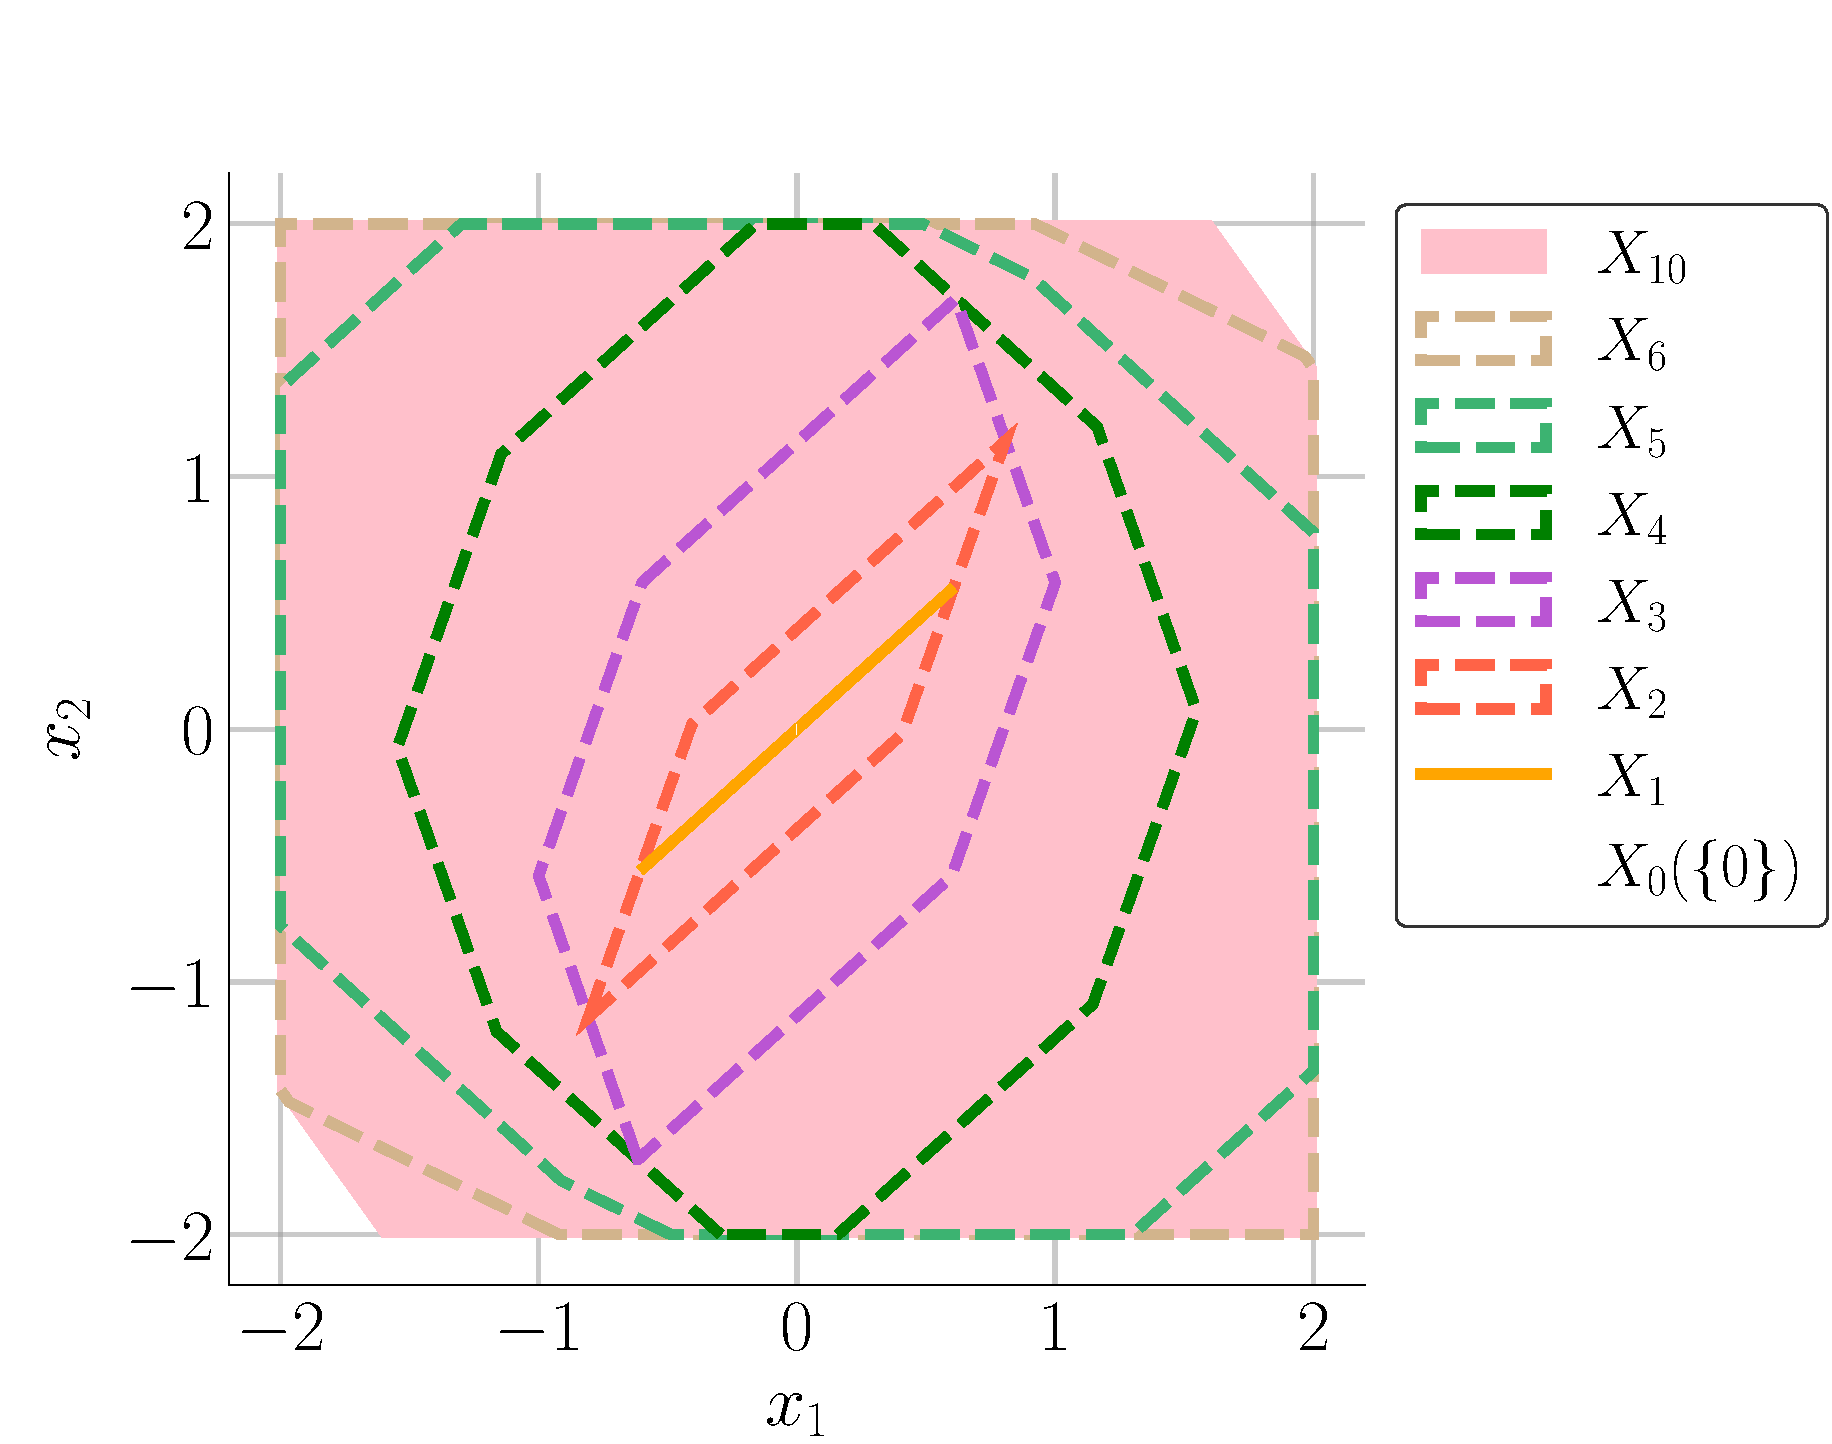
\includegraphics[width=0.45\linewidth]{figures/q3_i_X.pdf}}
    \quad
    \subfigure{
        \label{fig:q3_i_X_x}
        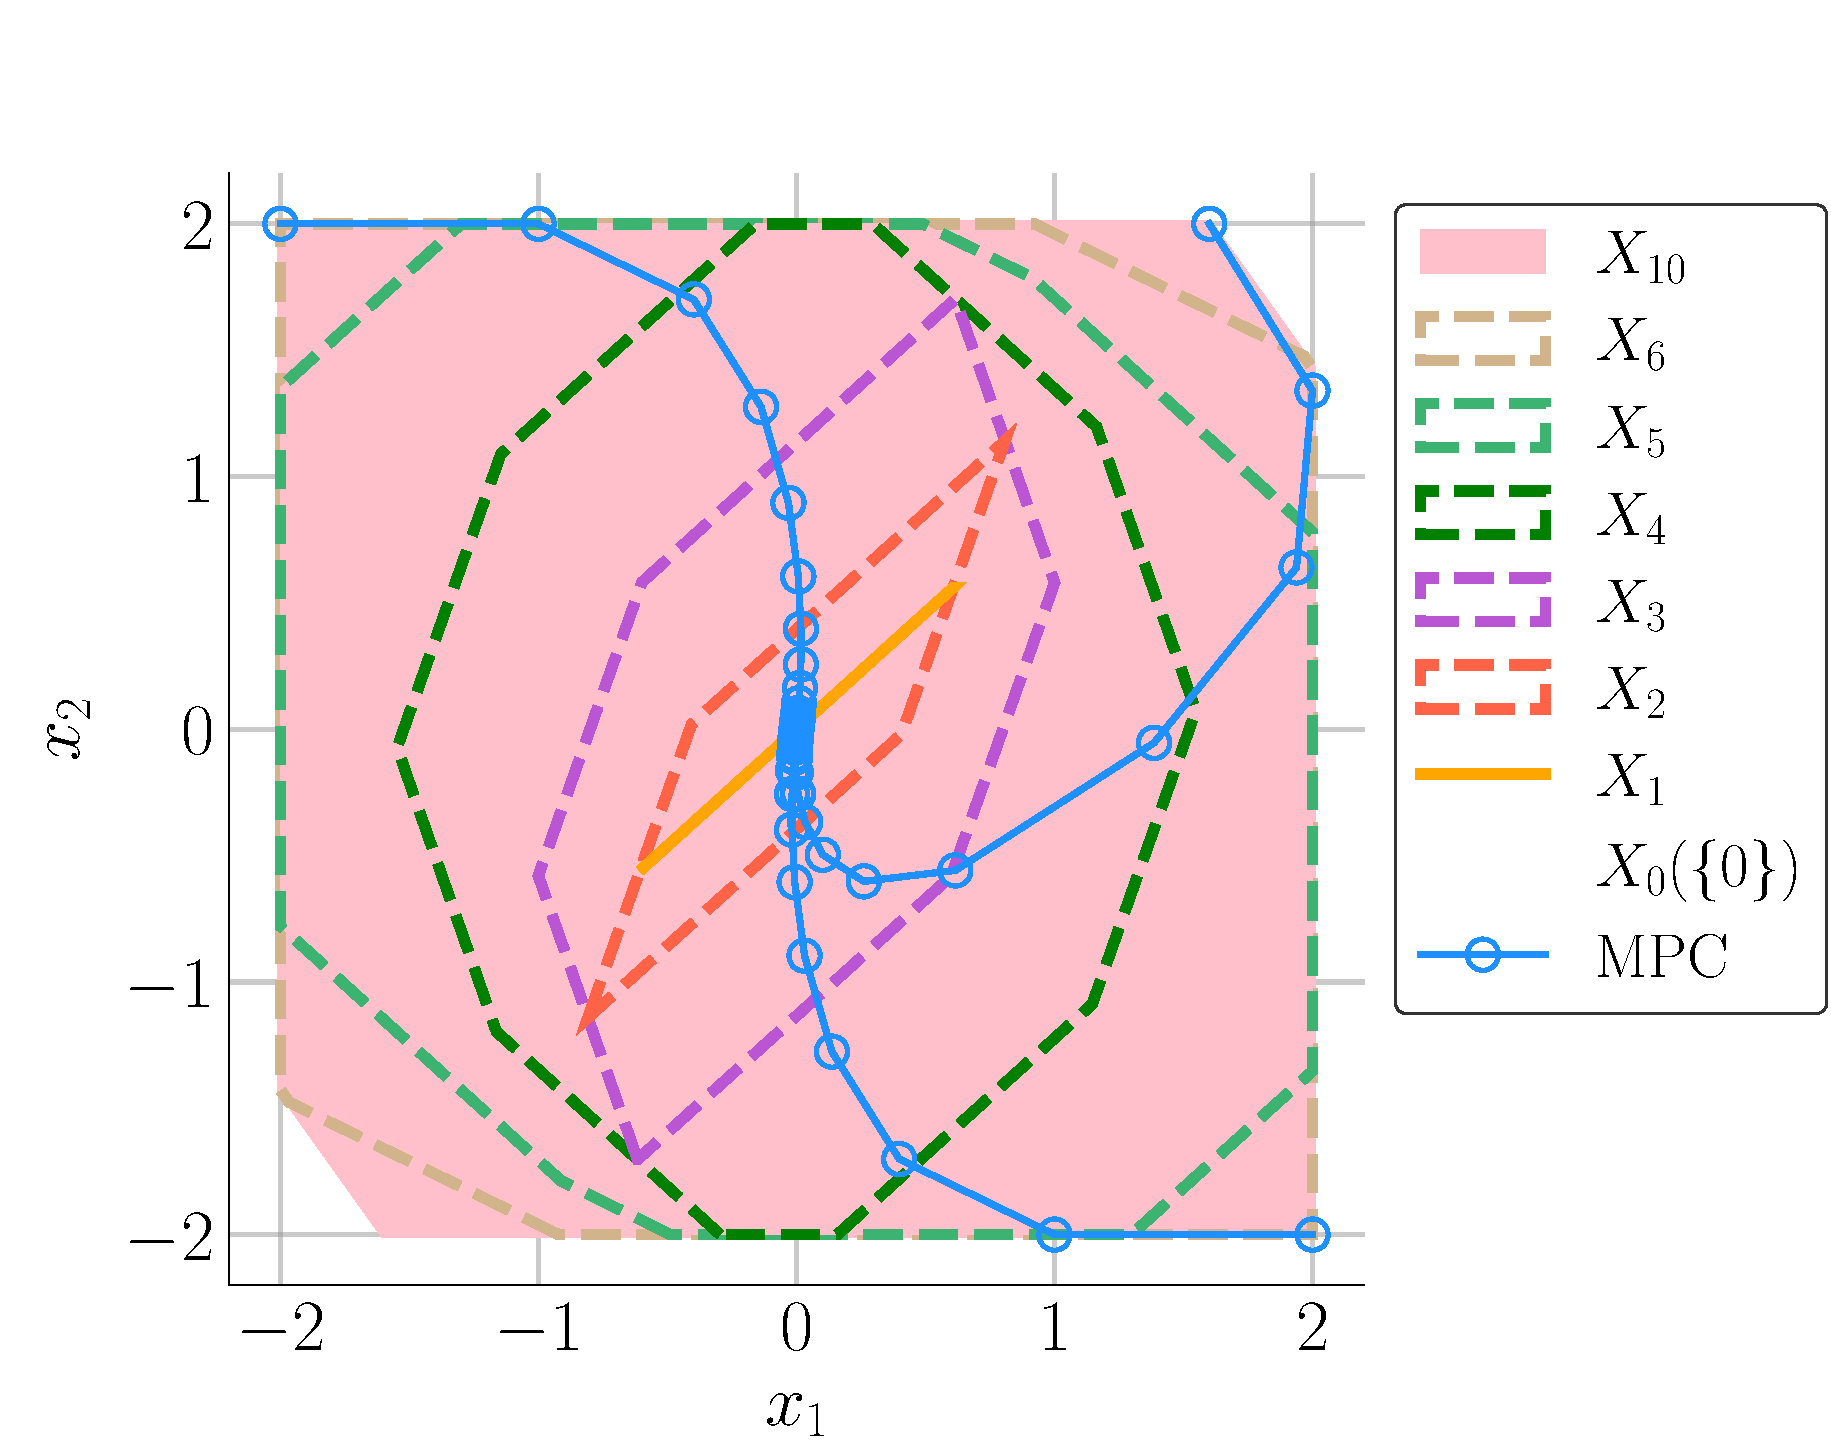
\includegraphics[width=0.45\linewidth]{figures/q3_i_X_x.pdf}}
    \caption{We denote by $X_t(X_f)$ the set of states that can be steered in no more than $t$
    steps to $X_f$. Observe that $Xt(\{0\})\subseteq Xt'(\{0\})$ for $t < t'$. In
    other words, the larger the terminal set or the larger the prediction horizon is, the larger
    the set of feasible states will be. In the right plot we see three trajectories of the
    MPC-controlled system with $N = 10$, starting from three extreme points of $X_{10}(\{0\})$. The extreme points are $\begin{bsmallmatrix}-2\\2\end{bsmallmatrix}, \begin{bsmallmatrix}1.6\\2\end{bsmallmatrix}, \begin{bsmallmatrix}2\\-2\end{bsmallmatrix}$. The set
    $X_0(\{0\})$ is shown in all plots.}
    \label{fig:q3_i_Xx}
\end{figure}
The simulation of the MPC-controlled dynamical system is shown in Figure \ref{fig:q3_i_xt_ut} and Figure \ref{fig:q3_i_cost} below.
\begin{figure}[H]
    \centering
    \vspace{-0.35cm}
    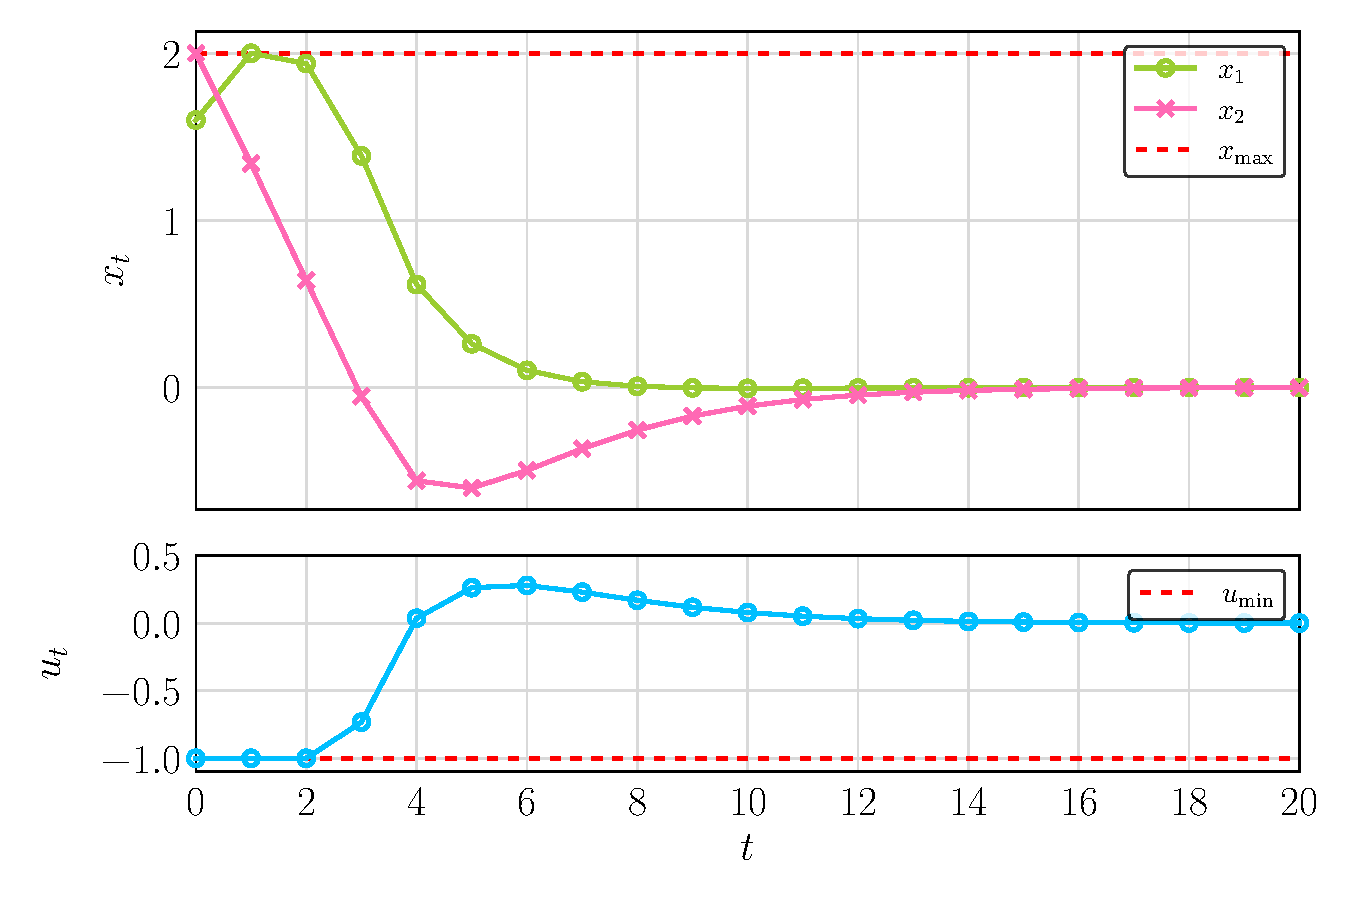
\includegraphics[width=0.7\linewidth]{figures/q3_i_xt_ut.pdf}
    \caption{In the above plot we see the states changing of the MPC-
    controlled system with $N = 10$, and in the below plot we see the control actions changing of the MPC-
    controlled system with $N = 10$, starting from the extreme point $\begin{bsmallmatrix}1.6\\2\end{bsmallmatrix}$. 
    We can observe that $x_t$ is steered in $20$ steps to $X_0(\{0\})$.}
    \label{fig:q3_i_xt_ut}
\end{figure}
\begin{figure}[H]
    \centering
    \vspace{-0.35cm}
    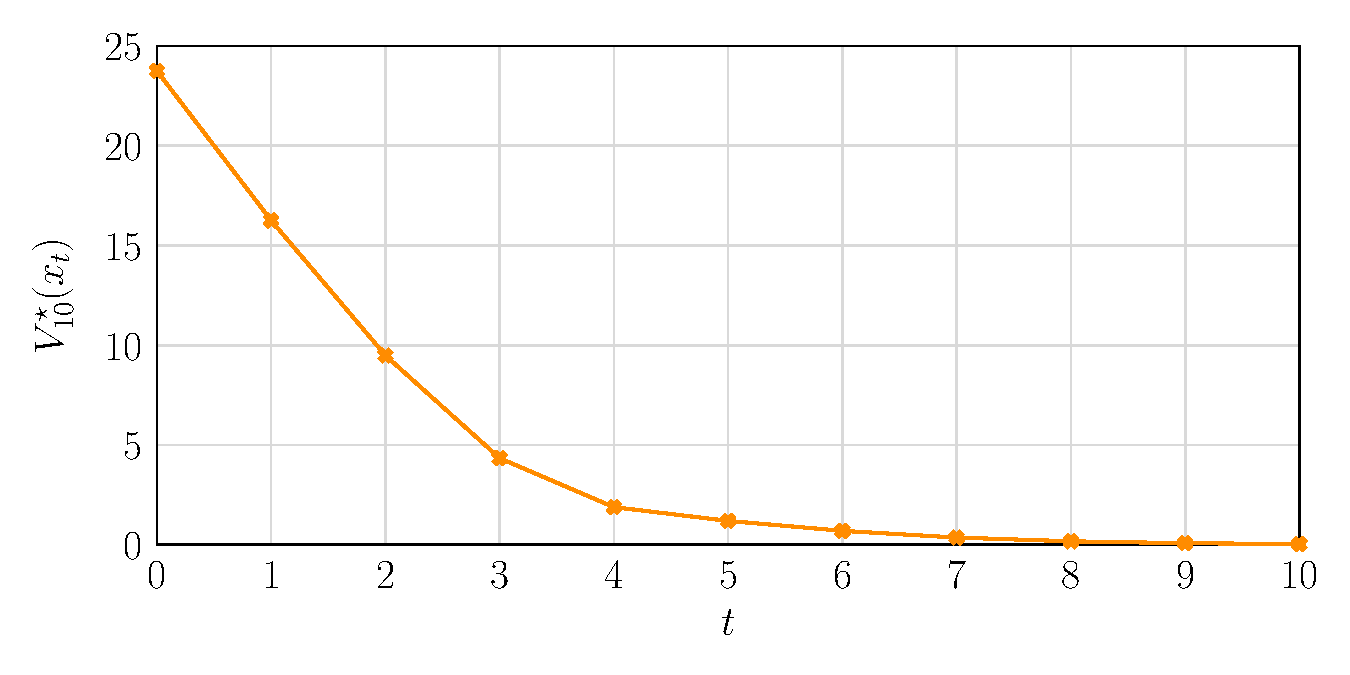
\includegraphics[width=0.7\linewidth]{figures/q3_i_cost.pdf}
    \caption{The ``energy'' of the system as measured by the Lyapunov function $V^{\star}_{10}$ for the MPC-controlled system with $N = 10$.}
    \label{fig:q3_i_cost}
\end{figure}
(ii) Design an MPC by following the procedure outlined in Handout 10, Sections 10.2 and 10.3. Use
a prediction horizon $N=10$ and compute the set of feasible states, $X_N$. Simulate the MPC-controlled
system starting from the extreme points of $X_N$.
\\ \\
\textbf{Answer:} 
The Python code: \href{https://github.com/Gczmy/ELE8088/blob/main/Coursework1/Python_code/3_ii.py}{Question 1.3 (ii)}.
\\
The MPC-controlled dynamical system with $N=10$, using one of the extreme points of $X_N$ as the initial state, $x_0=\begin{bsmallmatrix}\ \ 2\\-2\end{bsmallmatrix}$.
\\
MPC controller:
\begin{subequations}
    \begin{align}
        \mathbb{P}_N(x){}:{}
        \operatorname*{Minimise}_{\substack{u_0,u_1,\ldots,u_{N-1}\\ x_0,x_1,\ldots,x_N}}&\sum_{t=0}^{N-1} (\left\lVert x_t\right\rVert ^2_2+u_t^2),
        \\
        \text{subject to: }& x_{t+1} = 
        \begin{bsmallmatrix}
            1&0.7\\
            -0.1&1
        \end{bsmallmatrix}x_t + 
        \begin{bsmallmatrix}
            1\\
            0.5
        \end{bsmallmatrix}u_t, t\in\N_{[0,N-1]},
        \\
        &\begin{bsmallmatrix}
            -2\\
            -2
        \end{bsmallmatrix} 
        \leq x_t \leq 
        \begin{bsmallmatrix}
            2\\
            2
        \end{bsmallmatrix}, t\in\N_{[1,N]},
        \\
        &-1 \leq u_t \leq 1, t\in\N_{[0,N-1]},
        \\
        & x_0 = \begin{bsmallmatrix}\ \ 2\\-2\end{bsmallmatrix}.
    \end{align}
\end{subequations}
The set of feasible states is shown in Figure \ref{fig:q3_ii_Xx} below.
\begin{figure}[H]
    \centering
    \vspace{-0.35cm}
    \subfigtopskip=-2pt
    \subfigbottomskip=2pt
    \subfigcapskip=-5pt
    \subfigure{
        \label{fig:q3_ii_X}
        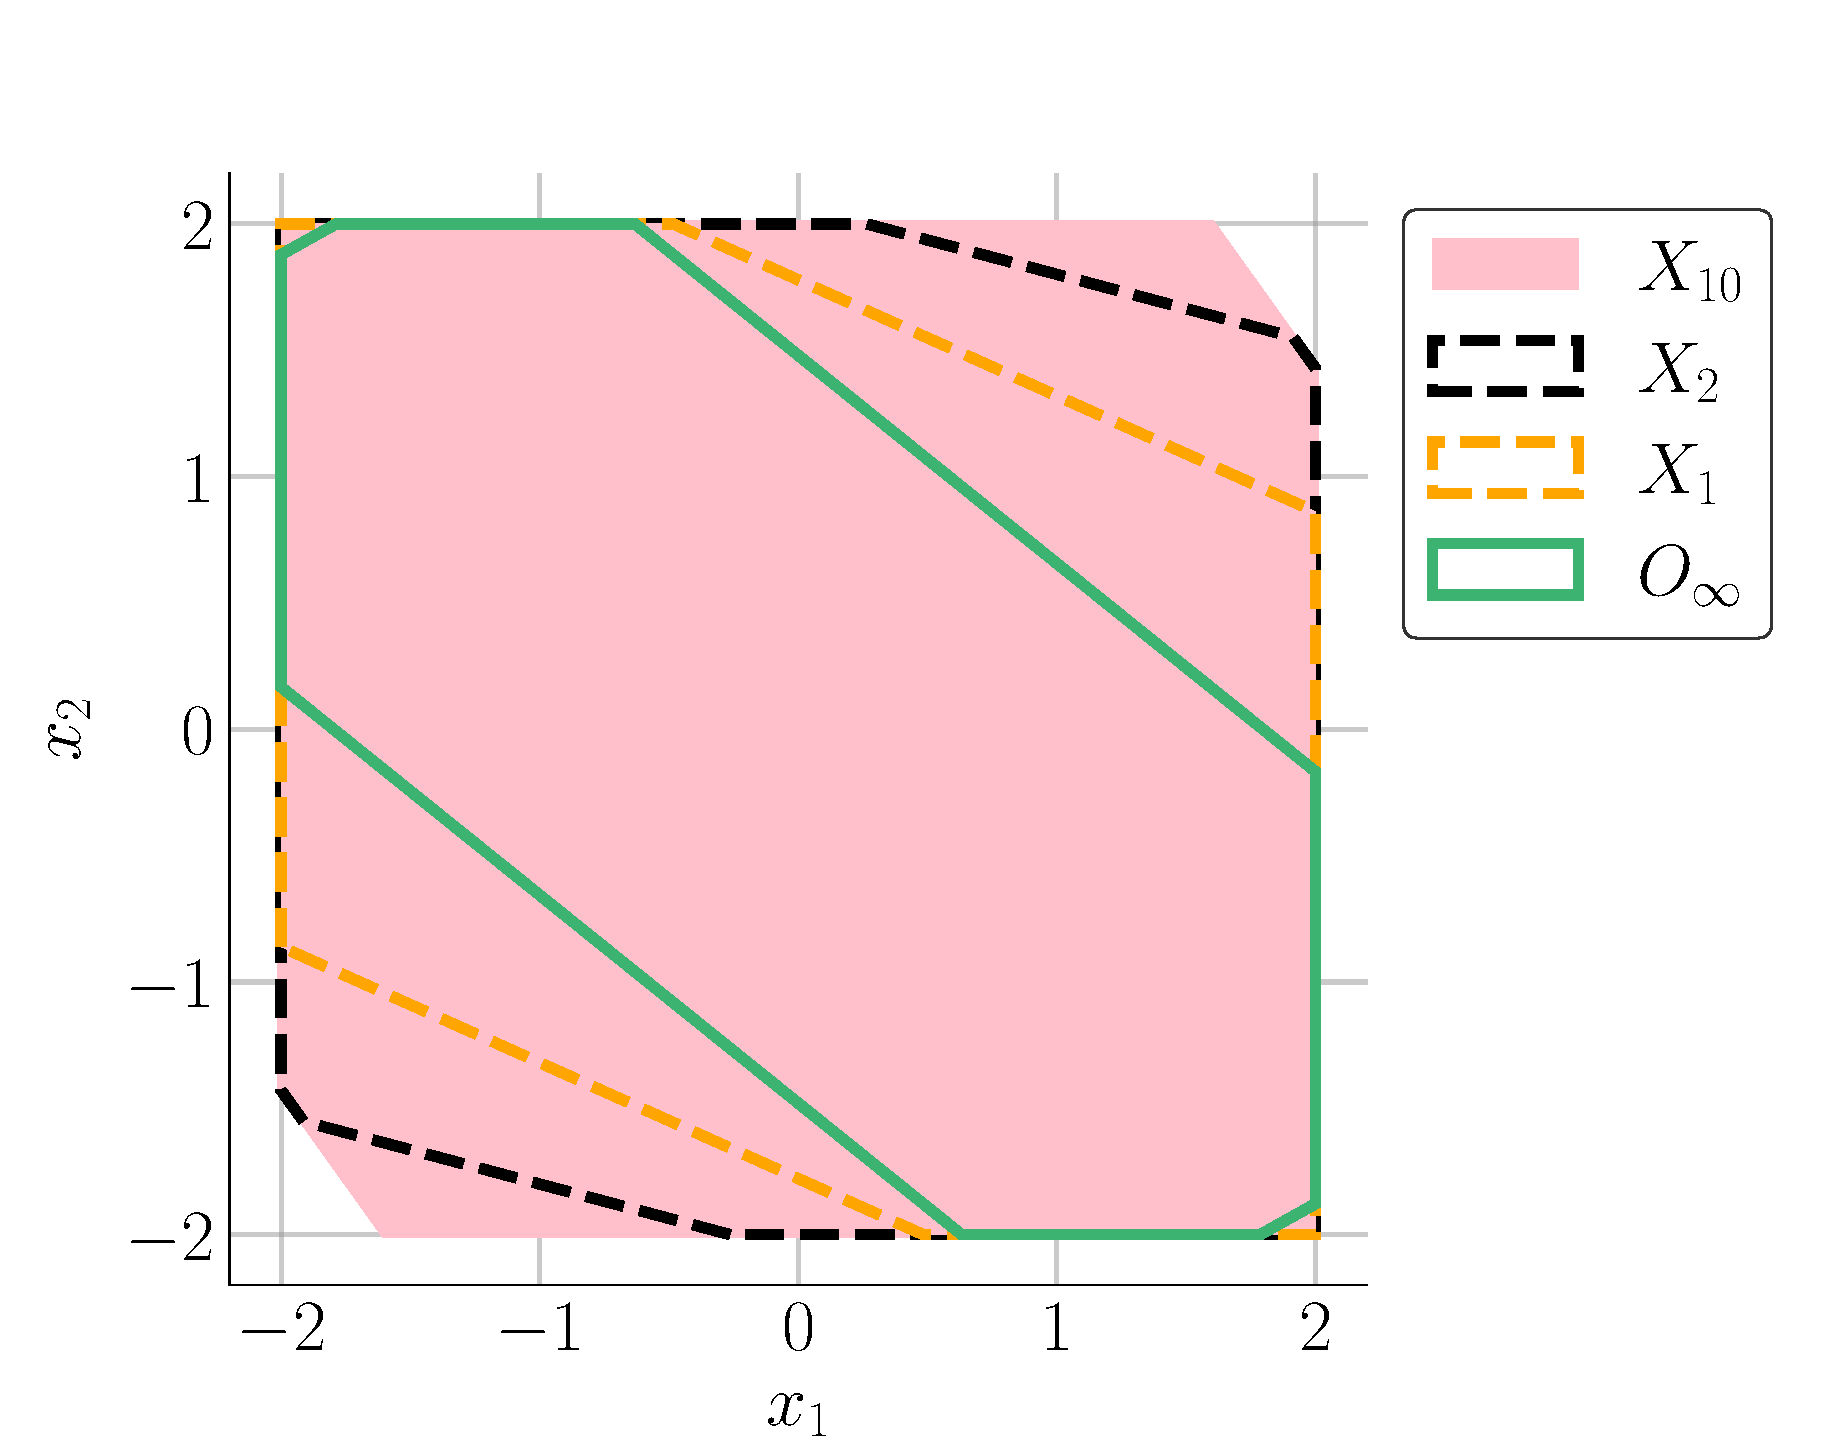
\includegraphics[width=0.47\linewidth]{figures/q3_ii_X.pdf}}
    \subfigure{
        \label{fig:q3_ii_X_x}
        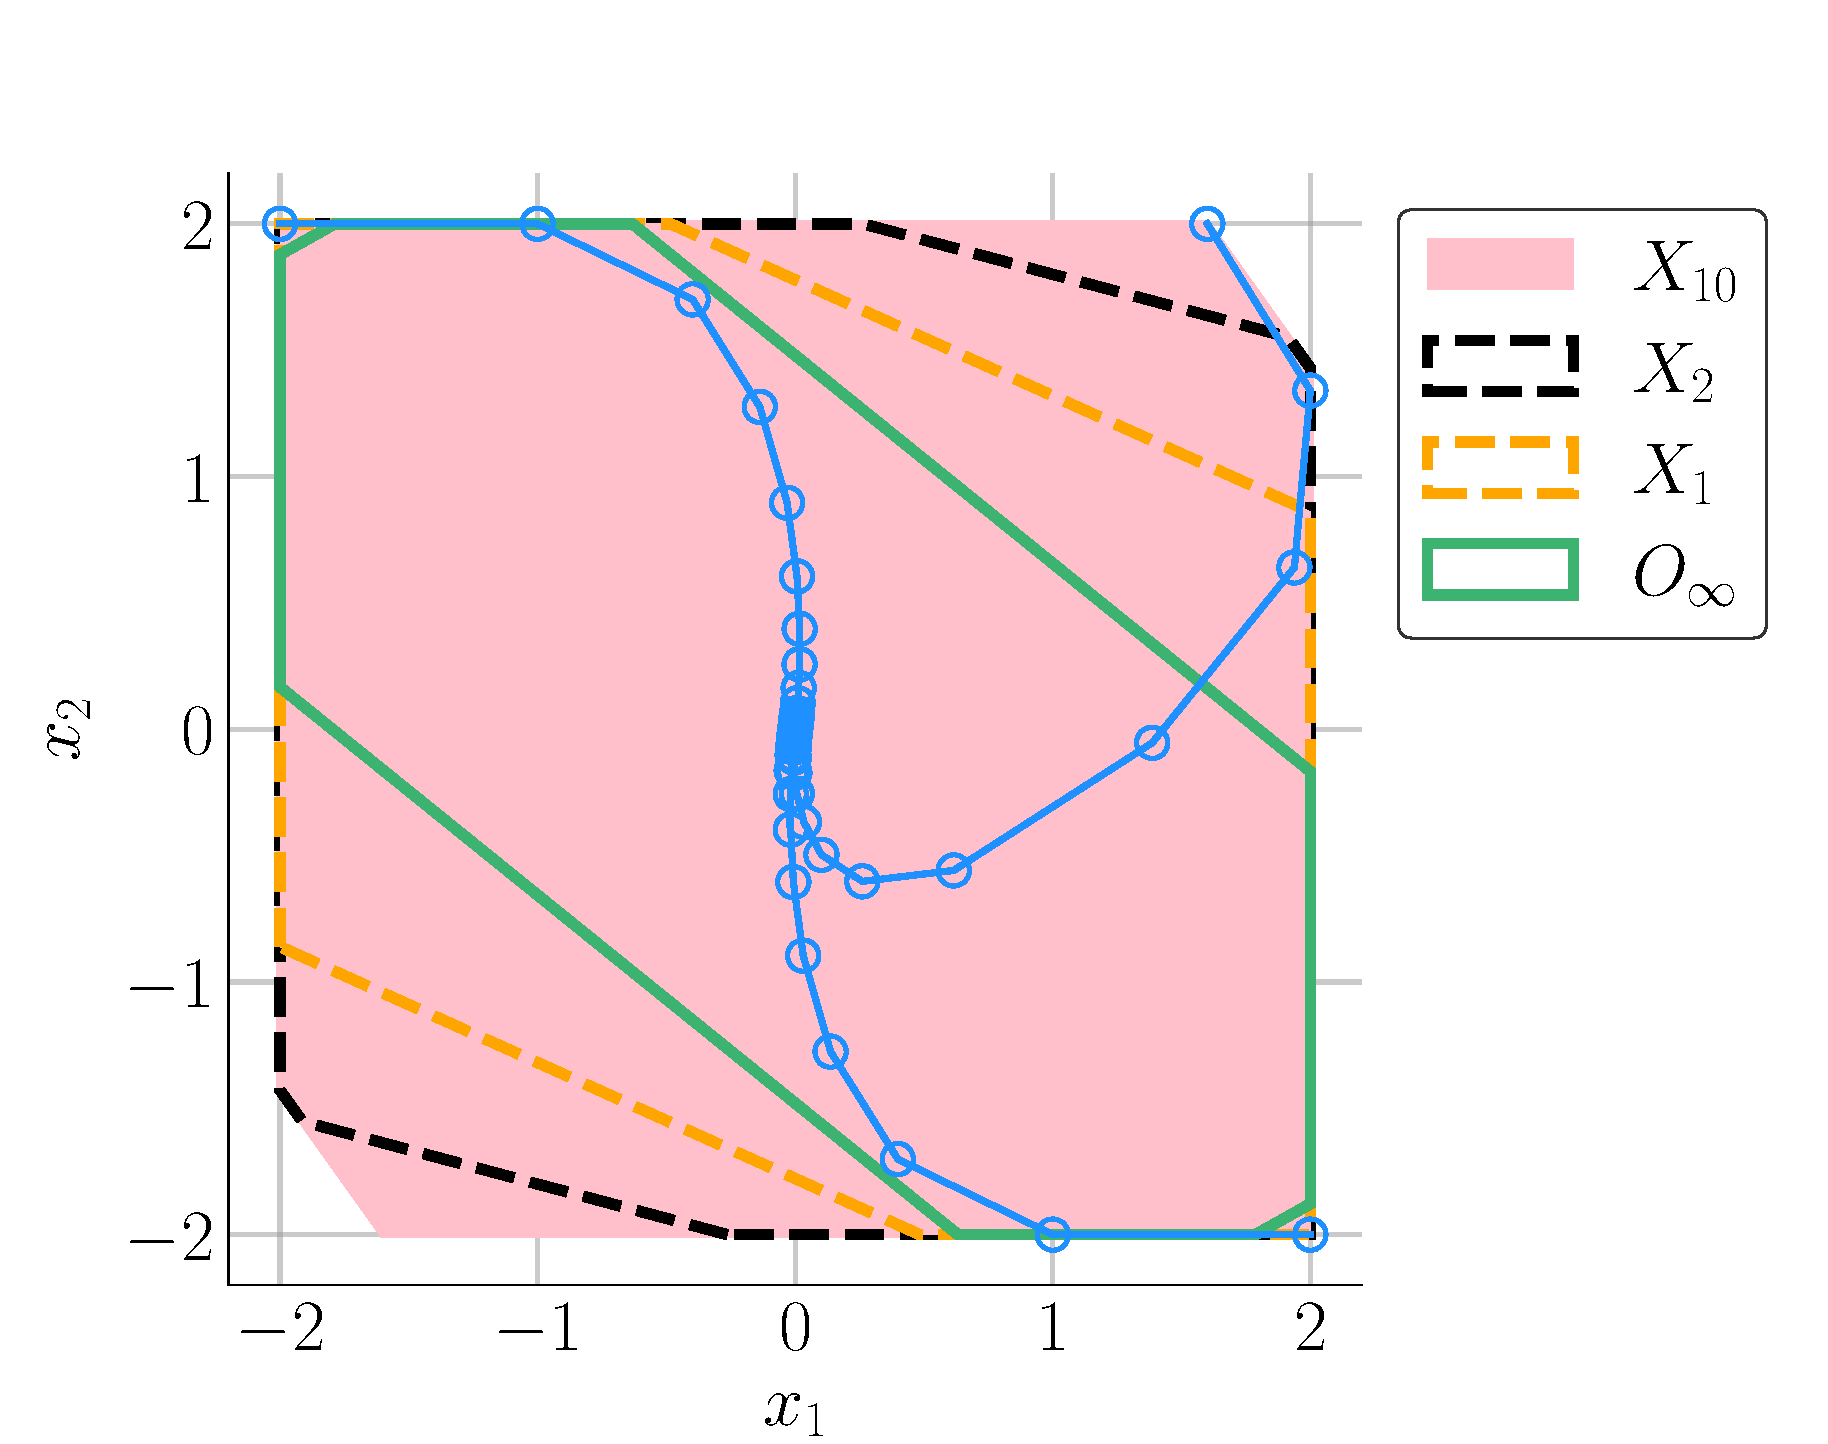
\includegraphics[width=0.47\linewidth]{figures/q3_ii_X_x.pdf}}
    \caption{We denote by $X_t(X_f)$ the set of states that can be steered in no more than $t$
    steps to $X_f$. Observe that $Xt(O_{\infty})\subseteq Xt'(O_{\infty})$ for $t < t'$. In
    other words, the larger the terminal set or the larger the prediction horizon is, the larger
    the set of feasible states will be. In the right plot we see three trajectories of the
    MPC-controlled system with $N = 10$, starting from three extreme points of $X_{10}(O_\infty)$. The extreme points are $\begin{bsmallmatrix}-2\\2\end{bsmallmatrix}, \begin{bsmallmatrix}1.6\\2\end{bsmallmatrix}, \begin{bsmallmatrix}2\\-2\end{bsmallmatrix}$. The set
    $O_{\infty}$ is shown in all plots with green colour.}
    \label{fig:q3_ii_Xx}
\end{figure}
The simulation of the MPC-controlled dynamical system is shown in Figure \ref{fig:q3_ii_xt_ut} and Figure \ref{fig:q3_ii_cost} below.
\begin{figure}[H]
    \centering
    \vspace{-0.35cm}
    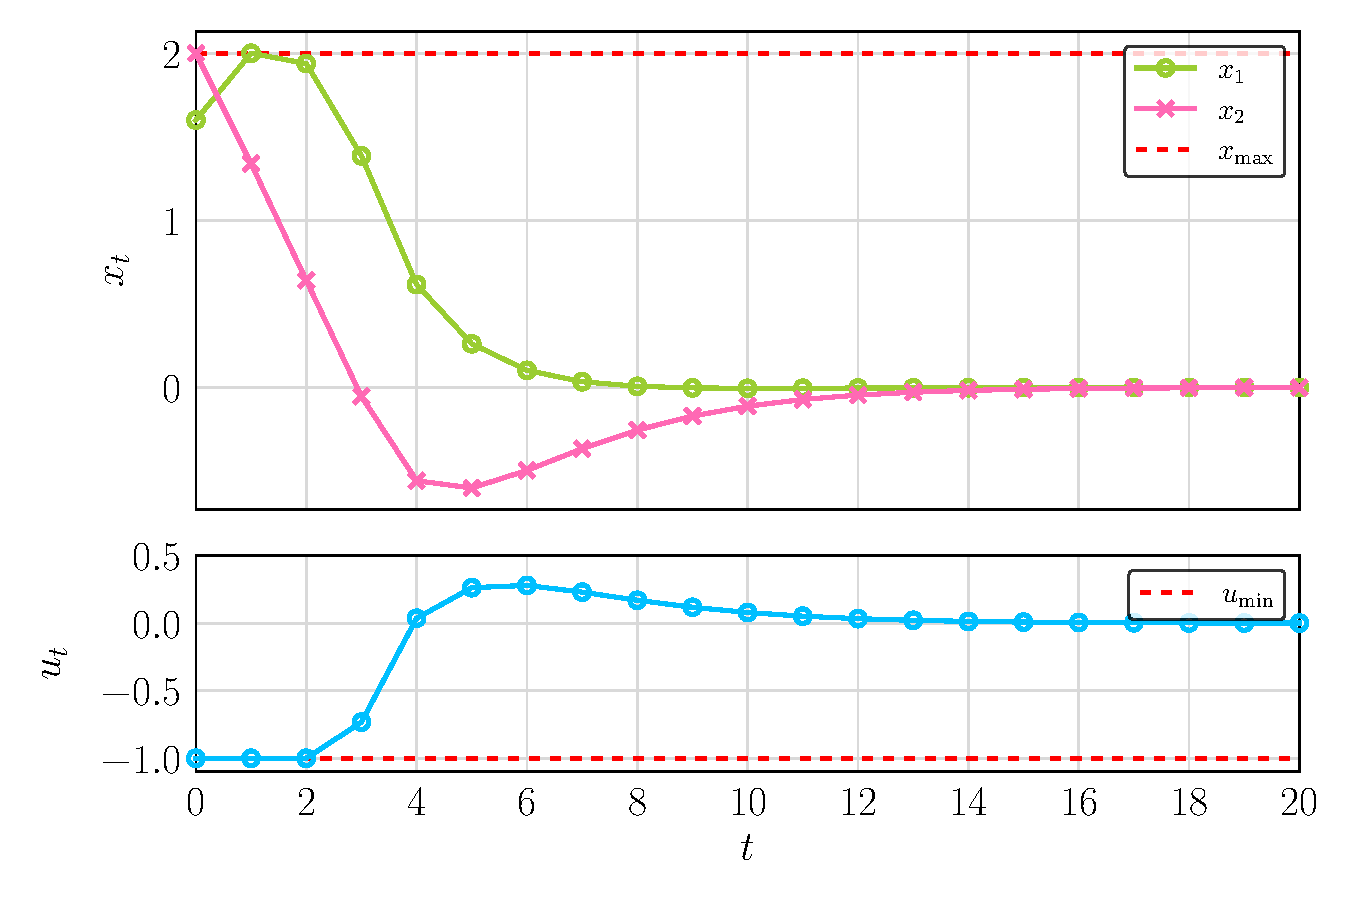
\includegraphics[width=0.7\linewidth]{figures/q3_ii_xt_ut.pdf}
    \caption{In the above plot we see the states changing of the MPC-
    controlled system with $N = 10$, and in the below plot we see the control actions changing of the MPC-
    controlled system with $N = 10$, starting from the extreme point $\begin{bsmallmatrix}1.6\\2\end{bsmallmatrix}$. 
    We can observe that $x_t$ is steered in $20$ steps to $O_{\infty}$.}
    \label{fig:q3_ii_xt_ut}
\end{figure}
\begin{figure}[H]
    \centering
    \vspace{-0.35cm}
    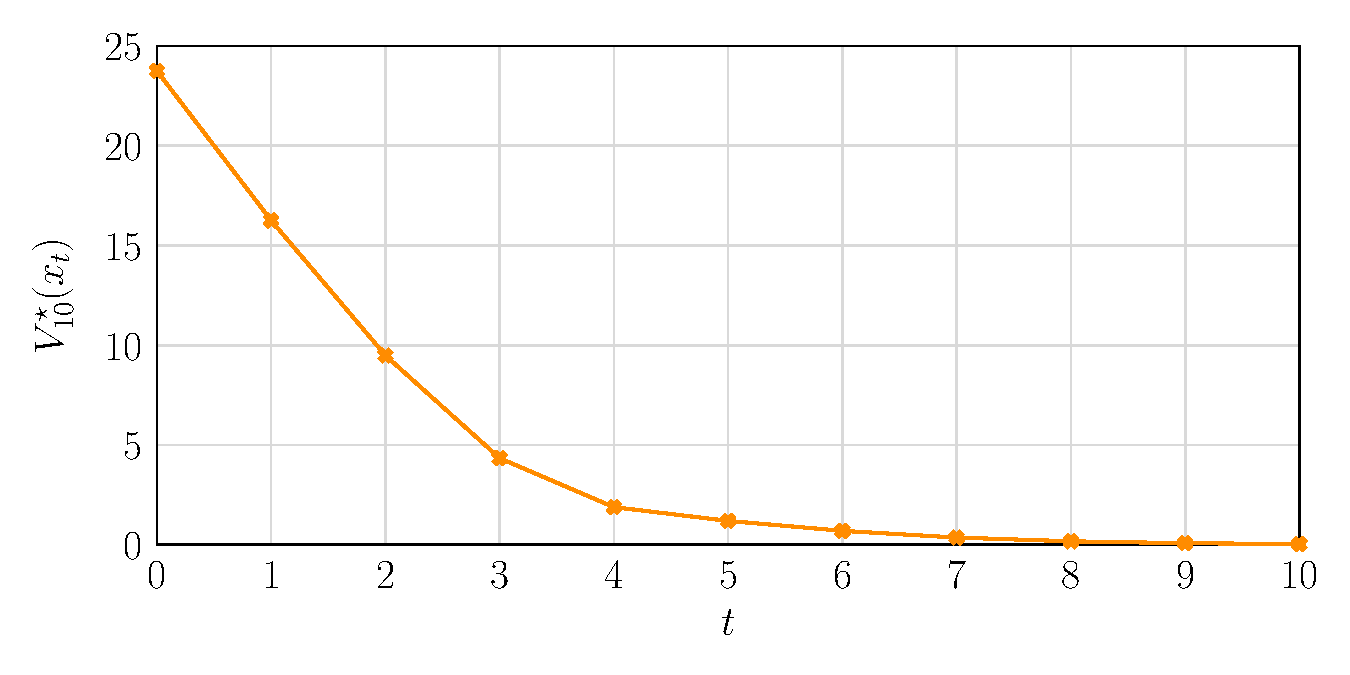
\includegraphics[width=0.7\linewidth]{figures/q3_ii_cost.pdf}
    \caption{The ``energy'' of the system as measured by the Lyapunov function $V^{\star}_{10}$ for the MPC-controlled system with $N = 10$.}
    \label{fig:q3_ii_cost}
\end{figure}
(iii) Design an MPC controller using an ellipsoidal terminal set and prediction horizon $N=10$. Provide simulation results starting from different initial states.
\\ \\
\textbf{Answer:} 
The Python code: \href{https://github.com/Gczmy/ELE8088/blob/main/Coursework1/Python_code/3_iii.py}{Question 1.3 (iii)}.
\\
Using an ellipsoidal terminal set, let
\begin{equation}
    \alpha \leq \min_{i\in\N_{[1,s]}}\frac{b_i^2}{\|P^{-1/2}h_i\|_2^2}
\end{equation}
MPC controller:
\begin{subequations}
    \begin{align}
        \mathbb{P}_N(x){}:{}
        \operatorname*{Minimise}_{\substack{u_0,u_1,\ldots,u_{N-1}\\ x_0,x_1,\ldots,x_N}}&\sum_{t=0}^{N-1} (\left\lVert x_t\right\rVert ^2_2+u_t^2) + \tfrac{1}{2}x_N^{\tran}P x_N,
        \\
        \text{subject to: }& x_{t+1} = 
        \begin{bsmallmatrix}
            1&0.7\\
            -0.1&1
        \end{bsmallmatrix}x_t + 
        \begin{bsmallmatrix}
            1\\
            0.5
        \end{bsmallmatrix}u_t, t\in\N_{[0,N-1]},
        \\
        &x_N^{\tran} P x_N \leq \alpha,
        \\
        &\begin{bsmallmatrix}
            -2\\
            -2
        \end{bsmallmatrix} 
        \leq x_t \leq 
        \begin{bsmallmatrix}
            2\\
            2
        \end{bsmallmatrix}, t\in\N_{[1,N]},
        \\
        &-1 \leq u_t \leq 1, t\in\N_{[0,N-1]},
        \\
        & x_0 = x.
    \end{align}
\end{subequations}
The simulation of the MPC-controlled dynamical system is shown in Figure \ref{fig:q3_iii_xt_ut} and Figure \ref{fig:q3_iii_cost} below.
\begin{figure}[H]
    \centering
    \vspace{-0.35cm}
    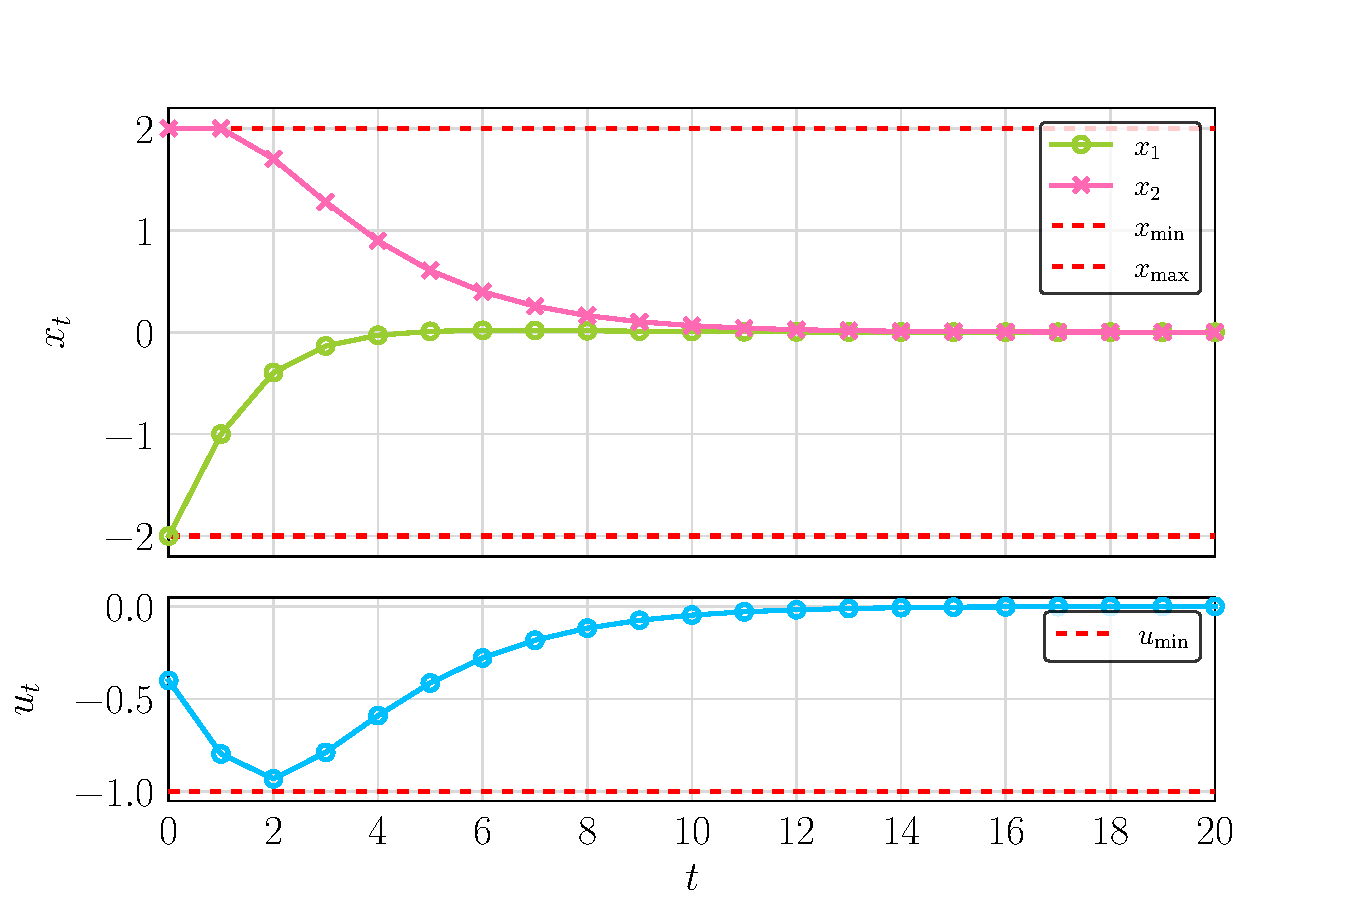
\includegraphics[width=0.7\linewidth]{figures/q3_iii_xt_ut.pdf}
    \caption{In the above plot we see the states changing of the MPC-
    controlled system with $N = 10$, and in the below plot we see the control actions changing of the MPC-
    controlled system with $N = 10$, starting from the extreme point $\begin{bsmallmatrix}-2\\2\end{bsmallmatrix}$. 
    We can observe that $x_t$ is steered in $20$ steps to $X_f$.}
    \label{fig:q3_iii_xt_ut}
\end{figure}
\begin{figure}[H]
    \centering
    \vspace{-0.35cm}
    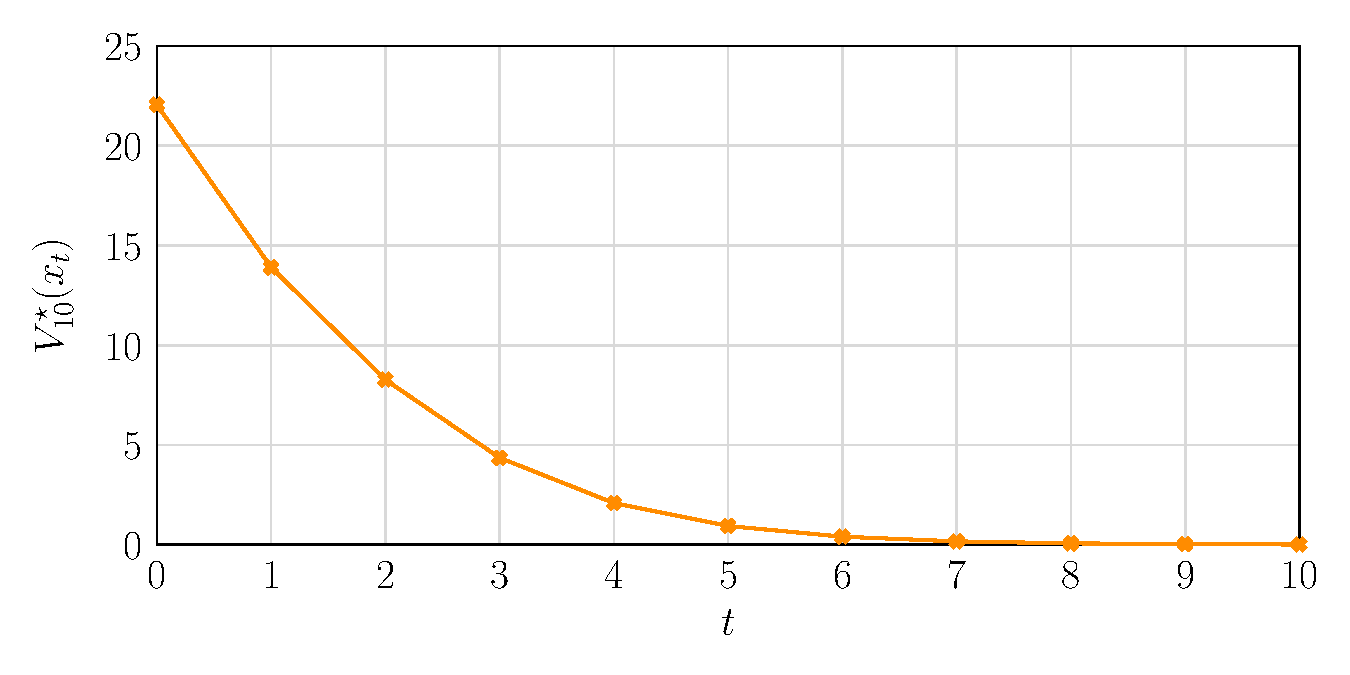
\includegraphics[width=0.7\linewidth]{figures/q3_iii_cost.pdf}
    \caption{The ``energy'' of the system as measured by the Lyapunov function $V^{\star}_{10}$ for the MPC-controlled system with $N = 10$.}
    \label{fig:q3_iii_cost}
\end{figure}
Now consider the nonlinear dynamical system\footnote[2]{We denote the two coordinates of $x_t\in\R^2$ by $x_{t,1}$ and $x_{t,2}$}.
\begin{equation}
    x_{t+1}=
    \begin{bmatrix}
        1&0.7\\
        -0.1&1
    \end{bmatrix}
    x_t+
    \begin{bmatrix}
        1\\
        0.5
    \end{bmatrix}
    u_t+
    \frac{1}{20}
    \begin{bmatrix}
        x_t^{\tran}x_t\\
        \sin^2(x_{t,1})
    \end{bmatrix},
\end{equation}
which is subject to the constraints given in \eqref{eq:q2_constraints}.
\\ \\
(iv) Design a nonlinear model predictive controller using the methodology of Section 10.6 in Handout 10: determine the terminal cost function and the terminal set of constraints.
\\ \\
\textbf{Answer:} 
The Python code: \href{https://github.com/Gczmy/ELE8088/blob/main/Coursework1/Python_code/3_iv.py}{Question 1.3 (iv)}.
\\
Choose $\ell(x,u)=\tfrac{1}{2}(x^{\tran}Qx+u^{\tran}Ru)=\left\lVert x\right\rVert ^2_2+u^2$, hence $Q=\begin{bsmallmatrix}\sqrt{2}&0\\0&\sqrt{2}\end{bsmallmatrix},R=\sqrt{2}.$
Let $K$ be a stabilising gain for $(A, B)$. Define $\bar{A} = A + BK, \bar{Q} = Q + K^{\tran}RK$. Choose $P\in\mathbb{S}^2_{++}$ such that
\begin{equation}
    P=\bar{A}^{\tran}P\bar{A}+2\bar{Q}.
\end{equation}
Calculate it by Python, we can get
\begin{equation}
    P=
    \begin{bmatrix}
        5.95663&-1.17022\\
        -1.17022&6.60196
    \end{bmatrix}.
\end{equation}
Choose $V_f(x)=\tfrac{1}{2}x^{\tran}Px$ and $X_f=\{x\in\R^2:V_f(x)\leq\tfrac{\alpha}{2}\}$, for appropriately small $\alpha>0$.
\\
We can get the terminal cost function
\begin{equation}
    V_f(x)=\frac{1}{2}x^{\tran}
    \begin{bmatrix}
        5.95663&-1.17022\\
        -1.17022&6.60196
    \end{bmatrix}x.
\end{equation}
\begin{align}
    X_f&=\{x\in\R^2:V_f(x)\leq\tfrac{\alpha}{2}\}
    \notag\\
    &=\{x\in\R^2:x^{\tran}Px\leq\alpha\}
\end{align}
NMPC controller:
\begin{subequations}
    \begin{align}
        \mathbb{P}_N(x){}:{}
        \operatorname*{Minimise}_{\substack{u_0,u_1,\ldots,u_{N-1}\\ x_0,x_1,\ldots,x_N}}&\sum_{t=0}^{N-1} (\left\lVert x_t\right\rVert ^2_2+u_t^2) + \tfrac{1}{2}x_N^{\tran}\begin{bsmallmatrix}5.95663&-1.17022\\-1.17022&6.60196\end{bsmallmatrix}x_N,
        \\
        \text{subject to: }& x_{t+1} = 
        \begin{bsmallmatrix}
            1&0.7\\
            -0.1&1
        \end{bsmallmatrix}x_t + 
        \begin{bsmallmatrix}
            1\\
            0.5
        \end{bsmallmatrix}u_t+
        \tfrac{1}{20}
        \begin{bsmallmatrix}
            x_t^{\tran}x_t\\
            \sin^2(x_{t,1})
        \end{bsmallmatrix}, t\in\N_{[0,N-1]},
        \\
        &x_N^{\tran} P x_N \leq \alpha,
        \\
        &\begin{bsmallmatrix}
            -2\\
            -2
        \end{bsmallmatrix} 
        \leq x_t \leq 
        \begin{bsmallmatrix}
            2\\
            2
        \end{bsmallmatrix}, t\in\N_{[1,N]},
        \\
        &-1 \leq u_t \leq 1, t\in\N_{[0,N-1]},
        \\
        & x_0 = x.
    \end{align}
\end{subequations}
Calculate $\alpha$ by Python, we can get $\alpha=5.749210061145554$.
\\
Thus, we can get the terminal set of constraints
\begin{equation}
    X_f=\{x\in\R^2:x^{\tran}Px\leq 5.749210061145554\}.
\end{equation}

\bibliographystyle{IEEEtran}
\bibliography{References}
\end{document}
